\documentclass[conference]{IEEEtran}
\usepackage{amsmath,amssymb,booktabs,graphicx,url,multirow}
\usepackage{pgfplots}
\pgfplotsset{compat=1.18}
\begin{document}
\title{Tectonic IEEEtran Smoke Test}
\author{\IEEEauthorblockN{A. Author}}
\maketitle
\begin{abstract}
Testing IEEEtran with tectonic.
\end{abstract}
\section{Intro}
Equation:
\begin{equation}
\widetilde{\Sigma}_m = (I - P^{G}_m)\,\Sigma^{D}_m\,(I - P^{G}_m).
\end{equation}
\begin{table}[t]
\centering
\caption{Test table}
\begin{tabular}{lrr}
\toprule
Method & F1 & Params \\
\midrule
LoRA & 81.2 & 1.33M \\
DRIFT & 82.9 & 1.33M \\
\bottomrule
\end{tabular}
\end{table}

\begin{figure}[t]
\centering
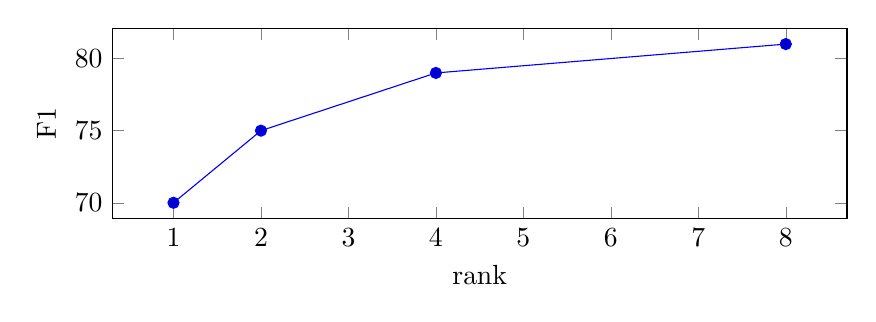
\begin{tikzpicture}
\begin{axis}[width=0.9\columnwidth,height=4cm,xlabel={rank},ylabel={F1}]
\addplot coordinates {(1,70) (2,75) (4,79) (8,81)};
\end{axis}
\end{tikzpicture}
\caption{Test plot}
\end{figure}
\end{document}
